\subsection{Plastic plate - von Mises plasticity (2D)}

\subsubsection*{Problem definition}

This is a typical plane strain benchmark for von Mises plasticity,
which is defined in \cite{SteEtAl:03}. We first analyze this example
to compare the behavior of two approaches on pure plastic
deformation problems. In the present simulation, a  quarter of plate
is taken due to the symmetry of the problem. The model set-up is
depicted in Fig. \ref{ex1_model}. The radius of the hole is 10$mm$.
Two points as point 1 and point 2 are specified to monitor the
evolution of variables. Point 1 is at  one third of the distance
from point 3 to point 4.

\begin{figure}[!htb]
\centering
    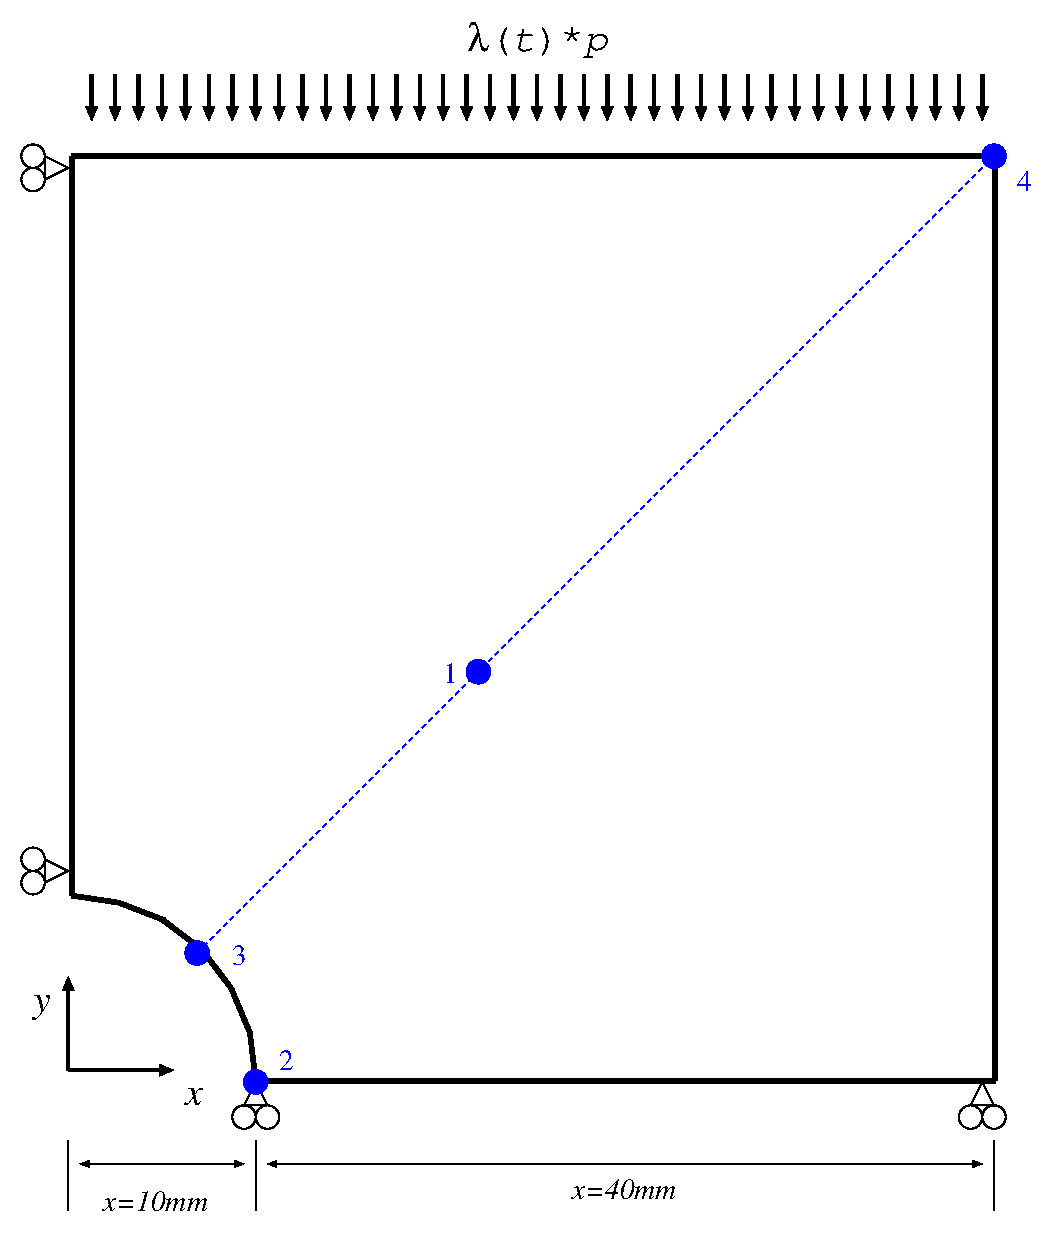
\includegraphics[scale=0.3]{M/ex1_model.eps}\\
   \caption{Stretched steel plate with a hole: one quarter}
  \label{ex1_model}
\end{figure}

\subsubsection*{Boundary conditions}

Traction boundary condition, $p=100N/mm^2\lambda(t)$  is
prescribed on the top with $\lambda(t)$, the time dependent scaling
factor. The case of  cycling loading is investigated with a scaling
function depicted in Fig. \ref{ex1_load}, in which,
$\lambda_{max}=4.1$.

\begin{figure}[!thb]
\centering
    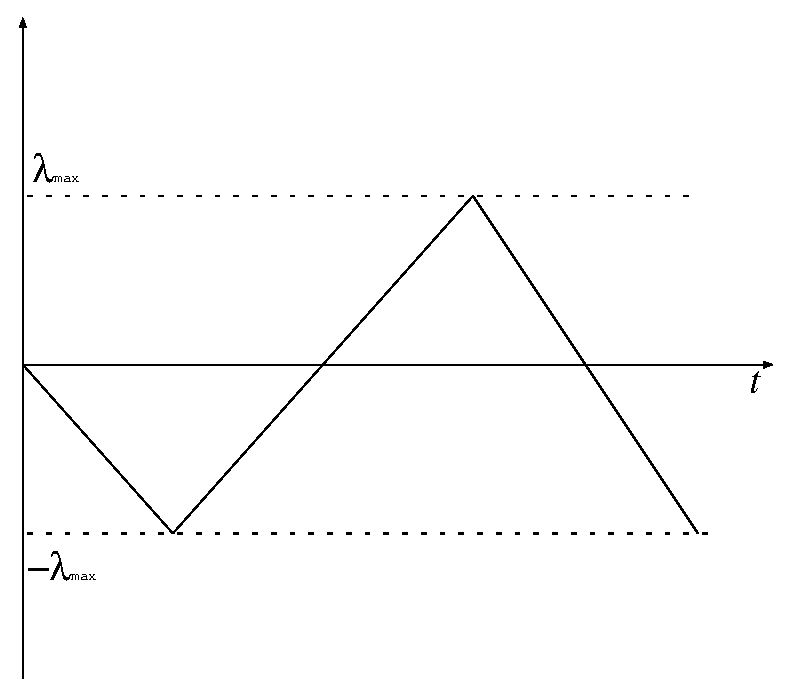
\includegraphics[scale=0.5]{M/ex1_load.eps}\\
   \caption{Time dependent load factor}
  \label{ex1_load}
\end{figure}

The domain is triangulated as depicted in Fig. \ref{ex1_mesh}.

\begin{figure}[!htb]
\centering
    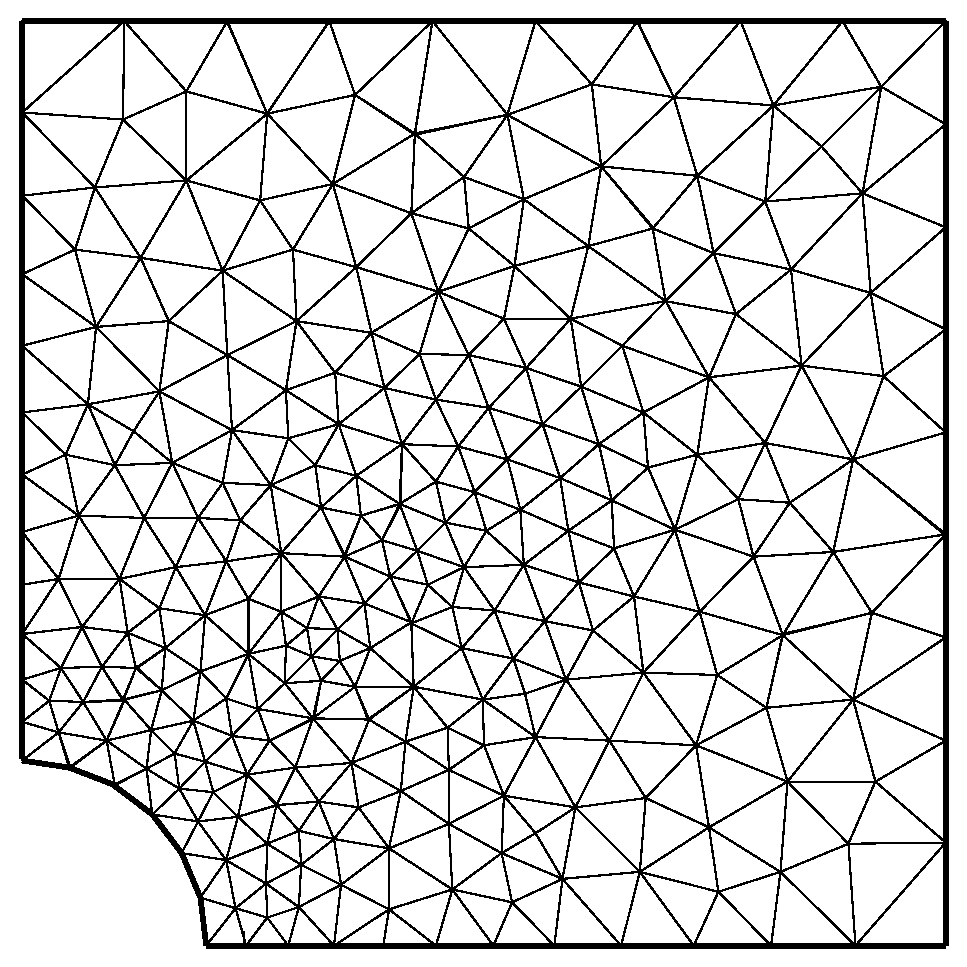
\includegraphics[scale=0.3]{M/ex1_mesh_gfem.eps}\\
   \caption{Mesh: 269 nodes and 484 elements}
  \label{ex1_mesh}
\end{figure}

\subsubsection*{Material properties}

The domain is assumed in homogeneous state. Table \ref{ex1_table1}
gives the material parameters\cite{SteEtAl:03}.

\begin{table}[!thb]
\centering
\caption{Material properties}
\label{ex1_table1}
\begin{tabular}{lll}
\hline\hline\noalign{\smallskip}
Property & Value & Unit \\
\noalign{\smallskip}\hline\noalign{\smallskip}
Young's modulus & $206900$  & $N/mm^2$ \\
Poisson's ratio & $0.29$       & $-$ \\
Initial yield stress & $450$       & $N/mm^2$ \\
Hardening modulus & $0.0$       & $kPa$ \\
\noalign{\smallskip}\hline\hline
\end{tabular}
\end{table}

\subsubsection*{Results}

The loading takes 60 steps with constant increment of
$\lambda_{max}/10$.  The similar distribution of plastic strain and
vertical stain given in Fig.\ref{ex2_cont1} shows implies the
behavior of von Mises plasticity.

%Contour plot
\begin{figure}[!thb]
  \begin{center}
   \begin{minipage}[t]{0.48\textwidth}
     \begin{center}
    \includegraphics[scale=0.28]{M/ex1_pls_4.1.eps}
    \centerline{(Plastic strain)}
    \end{center}
   \end{minipage}
   \hspace{0.02\textwidth}
   \begin{minipage}[t]{0.48\textwidth}
    \begin{center}
    \includegraphics[scale=0.28]{M/ex1_strain_yy_4.1.eps}\\
    \centerline{(Vertical strain)}
    \end{center}
   \end{minipage}\\
   %
  \end{center}
  \caption{Distribution of plastic strain and vertical strain at $\lambda_{max}/10$}
  \label{ex2_cont1}
\end{figure}

The evolution of horizontal displacements at point 1 and point 2
along with periodic load factor $\lambda (t)$ are shown on Fig.

\ref{ex2_loadp}.
\begin{figure}[!htb]
  \begin{center}
   \begin{minipage}[t]{0.48\textwidth}
     \begin{center}
    \includegraphics[scale=0.28]{M/ex1_load_v_ux_p1.eps}
    \centerline{(Point 1)}
    \end{center}
   \end{minipage}
   \hspace{0.02\textwidth}
   \begin{minipage}[t]{0.48\textwidth}
    \begin{center}
    \includegraphics[scale=0.28]{M/ex1_load_v_ux_p2.eps}\\
    \centerline{(Point 2)}
    \end{center}
   \end{minipage}\\
   %
  \end{center}
  \caption{Evolution of horizontal displacement vs load factor}
  \label{ex2_loadp}
\end{figure}

\subsubsection*{Benchmark deposit}
\begin{tabular}{|l|l|l|}
  \hline
  Benchmark & Problem type & Path in benchmark deposit \\
  \hline
 \emph{m\_mises} & M & benchmarks\verb \M\ \\
  \hline
\end{tabular}
